% Options for packages loaded elsewhere
\PassOptionsToPackage{unicode}{hyperref}
\PassOptionsToPackage{hyphens}{url}
%
\documentclass[
  doc,floatsintext]{apa6}
\usepackage{amsmath,amssymb}
\usepackage{iftex}
\ifPDFTeX
  \usepackage[T1]{fontenc}
  \usepackage[utf8]{inputenc}
  \usepackage{textcomp} % provide euro and other symbols
\else % if luatex or xetex
  \usepackage{unicode-math} % this also loads fontspec
  \defaultfontfeatures{Scale=MatchLowercase}
  \defaultfontfeatures[\rmfamily]{Ligatures=TeX,Scale=1}
\fi
\usepackage{lmodern}
\ifPDFTeX\else
  % xetex/luatex font selection
\fi
% Use upquote if available, for straight quotes in verbatim environments
\IfFileExists{upquote.sty}{\usepackage{upquote}}{}
\IfFileExists{microtype.sty}{% use microtype if available
  \usepackage[]{microtype}
  \UseMicrotypeSet[protrusion]{basicmath} % disable protrusion for tt fonts
}{}
\makeatletter
\@ifundefined{KOMAClassName}{% if non-KOMA class
  \IfFileExists{parskip.sty}{%
    \usepackage{parskip}
  }{% else
    \setlength{\parindent}{0pt}
    \setlength{\parskip}{6pt plus 2pt minus 1pt}}
}{% if KOMA class
  \KOMAoptions{parskip=half}}
\makeatother
\usepackage{xcolor}
\usepackage{graphicx}
\makeatletter
\def\maxwidth{\ifdim\Gin@nat@width>\linewidth\linewidth\else\Gin@nat@width\fi}
\def\maxheight{\ifdim\Gin@nat@height>\textheight\textheight\else\Gin@nat@height\fi}
\makeatother
% Scale images if necessary, so that they will not overflow the page
% margins by default, and it is still possible to overwrite the defaults
% using explicit options in \includegraphics[width, height, ...]{}
\setkeys{Gin}{width=\maxwidth,height=\maxheight,keepaspectratio}
% Set default figure placement to htbp
\makeatletter
\def\fps@figure{htbp}
\makeatother
\setlength{\emergencystretch}{3em} % prevent overfull lines
\providecommand{\tightlist}{%
  \setlength{\itemsep}{0pt}\setlength{\parskip}{0pt}}
\setcounter{secnumdepth}{-\maxdimen} % remove section numbering
% Make \paragraph and \subparagraph free-standing
\ifx\paragraph\undefined\else
  \let\oldparagraph\paragraph
  \renewcommand{\paragraph}[1]{\oldparagraph{#1}\mbox{}}
\fi
\ifx\subparagraph\undefined\else
  \let\oldsubparagraph\subparagraph
  \renewcommand{\subparagraph}[1]{\oldsubparagraph{#1}\mbox{}}
\fi
\newlength{\cslhangindent}
\setlength{\cslhangindent}{1.5em}
\newlength{\csllabelwidth}
\setlength{\csllabelwidth}{3em}
\newlength{\cslentryspacingunit} % times entry-spacing
\setlength{\cslentryspacingunit}{\parskip}
\newenvironment{CSLReferences}[2] % #1 hanging-ident, #2 entry spacing
 {% don't indent paragraphs
  \setlength{\parindent}{0pt}
  % turn on hanging indent if param 1 is 1
  \ifodd #1
  \let\oldpar\par
  \def\par{\hangindent=\cslhangindent\oldpar}
  \fi
  % set entry spacing
  \setlength{\parskip}{#2\cslentryspacingunit}
 }%
 {}
\usepackage{calc}
\newcommand{\CSLBlock}[1]{#1\hfill\break}
\newcommand{\CSLLeftMargin}[1]{\parbox[t]{\csllabelwidth}{#1}}
\newcommand{\CSLRightInline}[1]{\parbox[t]{\linewidth - \csllabelwidth}{#1}\break}
\newcommand{\CSLIndent}[1]{\hspace{\cslhangindent}#1}
\ifLuaTeX
\usepackage[bidi=basic]{babel}
\else
\usepackage[bidi=default]{babel}
\fi
\babelprovide[main,import]{english}
% get rid of language-specific shorthands (see #6817):
\let\LanguageShortHands\languageshorthands
\def\languageshorthands#1{}
% Manuscript styling
\usepackage{upgreek}
\captionsetup{font=singlespacing,justification=justified}

% Table formatting
\usepackage{longtable}
\usepackage{lscape}
% \usepackage[counterclockwise]{rotating}   % Landscape page setup for large tables
\usepackage{multirow}		% Table styling
\usepackage{tabularx}		% Control Column width
\usepackage[flushleft]{threeparttable}	% Allows for three part tables with a specified notes section
\usepackage{threeparttablex}            % Lets threeparttable work with longtable

% Create new environments so endfloat can handle them
% \newenvironment{ltable}
%   {\begin{landscape}\centering\begin{threeparttable}}
%   {\end{threeparttable}\end{landscape}}
\newenvironment{lltable}{\begin{landscape}\centering\begin{ThreePartTable}}{\end{ThreePartTable}\end{landscape}}

% Enables adjusting longtable caption width to table width
% Solution found at http://golatex.de/longtable-mit-caption-so-breit-wie-die-tabelle-t15767.html
\makeatletter
\newcommand\LastLTentrywidth{1em}
\newlength\longtablewidth
\setlength{\longtablewidth}{1in}
\newcommand{\getlongtablewidth}{\begingroup \ifcsname LT@\roman{LT@tables}\endcsname \global\longtablewidth=0pt \renewcommand{\LT@entry}[2]{\global\advance\longtablewidth by ##2\relax\gdef\LastLTentrywidth{##2}}\@nameuse{LT@\roman{LT@tables}} \fi \endgroup}

% \setlength{\parindent}{0.5in}
% \setlength{\parskip}{0pt plus 0pt minus 0pt}

% Overwrite redefinition of paragraph and subparagraph by the default LaTeX template
% See https://github.com/crsh/papaja/issues/292
\makeatletter
\renewcommand{\paragraph}{\@startsection{paragraph}{4}{\parindent}%
  {0\baselineskip \@plus 0.2ex \@minus 0.2ex}%
  {-1em}%
  {\normalfont\normalsize\bfseries\itshape\typesectitle}}

\renewcommand{\subparagraph}[1]{\@startsection{subparagraph}{5}{1em}%
  {0\baselineskip \@plus 0.2ex \@minus 0.2ex}%
  {-\z@\relax}%
  {\normalfont\normalsize\itshape\hspace{\parindent}{#1}\textit{\addperi}}{\relax}}
\makeatother

\makeatletter
\usepackage{etoolbox}
\patchcmd{\maketitle}
  {\section{\normalfont\normalsize\abstractname}}
  {\section*{\normalfont\normalsize\abstractname}}
  {}{\typeout{Failed to patch abstract.}}
\patchcmd{\maketitle}
  {\section{\protect\normalfont{\@title}}}
  {\section*{\protect\normalfont{\@title}}}
  {}{\typeout{Failed to patch title.}}
\makeatother

\usepackage{xpatch}
\makeatletter
\xapptocmd\appendix
  {\xapptocmd\section
    {\addcontentsline{toc}{section}{\appendixname\ifoneappendix\else~\theappendix\fi\\: #1}}
    {}{\InnerPatchFailed}%
  }
{}{\PatchFailed}
\usepackage{csquotes}
\usepackage{placeins} 

\ifLuaTeX
  \usepackage{selnolig}  % disable illegal ligatures
\fi
\IfFileExists{bookmark.sty}{\usepackage{bookmark}}{\usepackage{hyperref}}
\IfFileExists{xurl.sty}{\usepackage{xurl}}{} % add URL line breaks if available
\urlstyle{same}
\hypersetup{
  pdftitle={Impressiveness and trust in science},
  pdflang={en-EN},
  hidelinks,
  pdfcreator={LaTeX via pandoc}}

\title{Impressiveness and trust in science}
\author{\textsuperscript{}}
\date{}


\shorttitle{Impressiveness and trust in science}

\affiliation{\vspace{0.5cm}\textsuperscript{} }

\abstract{%
XX
}



\begin{document}
\maketitle

\hypertarget{introduction}{%
\section{Introduction}\label{introduction}}

XX

We cite a paper like this (Cologna et al., n.d.).

XX

Why might people trust science without understanding it? There is a popular explanation as to why people do not trust science enough: the deficit model. According to the deficit model, people do not trust in science enough, because they do not know enough about it. Yet, survey data consistently shows that most people do trust science - although, indeed, they do not seem to know much about it. To explain this, we propose the lasting-impression account. According to the lasting-impression account, people are impressed by scientific findings, e.g.~because of their difficulty, their precision, and their degree of consensus. They infer that scientists are competent and, everything else equal, trustworthy. We suspect that these impressions persist more than specific scientific knowledge, and are more relevant for explaining trust in science.

\hypertarget{overview-of-experiments}{%
\section{Overview of experiments}\label{overview-of-experiments}}

Experiments one and two tested whether exposure to impressive scientific content increases trust in scientists. Experiment 3, tests if this trust in scientists persists, and if it persists more than specific knowledge about the content.

\hypertarget{experiment-1}{%
\section{Experiment 1}\label{experiment-1}}

The main goal of experiment one to see if exposure to impressive science content could enhance people's trust in scientists. We had the following hypotheses:

\textbf{H1a: Participants will perceive scientists as more competent than they did before after having read an impressive text about their discipline's findings, compared to when reading a basic text.}

\textbf{H1b: Across all conditions, participants who are more impressed by the text about a discipline will also tend to perceive the scientists of the discipline as more competent.}

\textbf{H2a: Participants will trust a discipline more than they did before after reading an impressive text about the discipline's findings, compared to when reading a basic text.}

\textbf{H2b: Across all conditions, participants who are more impressed by the text about a discipline will also tend to trust the scientists of the discipline more.}

We had the following research questions:

\textbf{RQ1: Do participants perceive to learn more from the texts in the impressive condition, compared to the basic condition?}

\textbf{RQ2: Do perceptions of consensus interact with the relationships proposed in the hypotheses, such that greater perceived consensus is a associated with a more positive relationship between impressiveness and trust/competence?}

\hypertarget{methods}{%
\subsection{Methods}\label{methods}}

\hypertarget{participants}{%
\subsubsection{Participants}\label{participants}}

We recruited 100 participants via Prolific. Two participants failed our attention check, resulting in a final sample of 98 participants (48 female, 50 male; \(age_\text{mean}\): 39.40, \(age_\text{sd}\): 13.23, \(age_\text{median}\): 36).

\hypertarget{procedure}{%
\subsubsection{Procedure}\label{procedure}}

After providing their consent to participate in the study, participants were given an attention check: ``Imagine you are playing video games with a friend and at some point your friend says:''I don't want to play this game anymore! To make sure that you read the instructions, please write the three following words''I pay attention'' in the box below. I really dislike this game, it's the most overrated game ever. Do you agree with your friend?``. We excluded all participants whose answer did not resemble''I pay attention''. Then, participants read the following instructions: ``You're going to read two texts about scientific discoveries, in two fields: archeology (the study of human activity through the recovery and analysis of material culture), and entomology (the study of insects). We ask you to read the texts, and then answer a few questions about them.'' Next, participants read vignettes about scientific findings in the disciplines of entomology and archaeology. We manipulated the impressiveness of the texts, so that there was one ``basic'' and one ``impressive'' version for each of the disciplines (see Table \ref{tab:exp1-stimuli}). Impressiveness varies within participants, but between disciplines: each participant sees an \texttt{impressive} version for one discipline, and a \texttt{basic} version for the other discipline. After each text, participants are asked several questions about the vignette and their perceptions of the scientists' trustworthiness.

\hypertarget{materials}{%
\subsubsection{Materials}\label{materials}}

\begin{longtable}[t]{>{\raggedright\arraybackslash}p{5em}>{\raggedright\arraybackslash}p{20em}>{\raggedright\arraybackslash}p{20em}}
\caption{\label{tab:exp1-stimuli}Stimuli of Experiment 1}\\
\toprule
 & Impressive & Basic\\
\midrule
Archeology & Archeologists, scientists who study human history and prehistory, are able to tell, from their bones, whether someone was male or female, how old they were, and whether they suffered from a wide range of diseases. Archeologists can now even tell at what age someone, dead for tens of thousands of years, stopped drinking their mother’s milk, from the composition of their teeth. 

Looking for patterns, archeologists can also understand how far our ancestors traveled, or how often they fought each other.

Archeologists can learn about the language that our ancestors or cousins might have had. For instance, the nerve that is used to control breathing is larger in humans than in apes, plausibly because we need more fine-grained control of our breathing in order to speak. As a result, the canal containing that nerve is larger in humans than in apes – and it is also enlarged in Neanderthals. 

We can also tell, from an analysis of the tools they made, that, like modern humans, most Neanderthals were right-handed. It’s thought that handedness is related to the evolution of language, another piece of evidence suggesting that Neanderthals likely possessed a form of language. & Archaeology is the science that studies human history and prehistory based on the analysis of objects from the past such as human bones, engravings, constructions, and various objects, from nails to bits of pots. This task requires a great deal of carefulness, because objects from the past need to often be dug out from the ground and cleaned, without destroying them in the process. 

Archeologists have been able to shed light on human history in all continents, from ancient Egypt to the Incas in Peru or the Khmers in Cambodia. 

Archaeologists have made some startling discoveries, such as the amazing animal paintings in the Lascaux caves, which have been shown to be at least 30000 years old. On that basis, archeologists speculate on the artistic and religious lives of our ancestors. 

Archeologists have also been able to find remains of our more distant ancestors, showing that our species is just one among several that appeared and then went extinct, such as Neanderthals, Homo erectus, or Homo habilis. 

Archaeology relies on scientific methods of analysis such as carbon dating, which enables us to date objects, based on the type of carbon atoms they contain.\\
Entomology & Entomologists are the scientists who study insects. Some of them have specialized in understanding how insects perceive the world around them, and they have uncovered remarkable abilities. 

Entomologists interested in how flies’ visual perception works have used special displays to present images for much less than the blink of an eye, electrodes to record how individual cells in the flies’ brain react, and ultra-precise electron microscopy to examine their eyes. Thanks to these techniques, they have shown that some flies can perceive images that are displayed for just three milliseconds (a thousandth of a second) – about ten times shorter than a single movie frame (of which there are 24 per second). 

Entomologists who study the hair of crickets have shown that these microscopic hairs, which can be found on antenna-like organs attached to the crickets’ rear, are maybe the most sensitive organs in the animal kingdom. The researchers used extremely precise techniques to measure how the hair reacts to stimuli, such as laser-Doppler velocimetry, a technique capable of detecting the most minute of movements. They were able to show that the hair could react to changes in the motion of the air that had less energy than one particle of light, a single photon. & Entomologists are scientists who investigate insects, typically having a background in biology. They study, for example, how a swarm of bees organizes, or how ants communicate with each other. 

They also study how different insects interact with each other and their environment, whether some species are in danger of going extinct, or whether others are invasive species that need to be controlled.

Sometimes entomologists study insects by observing them in the wild, sometimes they conduct controlled experiments in laboratories, to see for example how different environmental factors change the behavior of insects, or to track exactly the same insects over a longer period of time.

An entomologist often specializes in one type of insect in order to study it in depth. For example, an entomologist who specializes in ants is called a myrmecologist.\\
\bottomrule
\end{longtable}

We asked participants how much they think they learned from reading the text (``How much do you feel you've learnt about human history by reading this text?'' {[}1 - Nothing, 2 - A bit, 3 - Some, 4 - Quite a bit, 5 - A lot{]}) and how impressive they found it (``How impressive do you think the findings of the archaeologists described in the text are?'' {[}1 - Not very impressive, 2 - A bit impressive, 3 - Quite impressive, 4 - Very impressive, 5 - Extremely impressive{]}). We also asked them about whether reading the text changed their impression of the competence of the scientists of the respective discipline (``Would you agree that reading this text has made you think of archaeologists as more competent than you thought before?'' {[}1 - Strongly disagree, 2 - Disagree, 3 - Neither agree nor disagree, 4 - Agree, 5 - Strongly agree{]}) and their trust in the respective discipline (``Having read this text, would you agree that you trust the discipline of archaeology more than you did before?'' {[}1 - Strongly disagree, 2 - Disagree, 3 - Neither agree nor disagree, 4 - Agree, 5 - Strongly agree{]}). Finally, we also asked about the perceived consensus (``To which extent do you think the findings from the short text you just read reflect a minority or a majority opinion among archaeologists?'' {[}1 - Small minority, 2 - Minority, 3 - About half, 4 - Majority, 5 - Large majority{]}).

\hypertarget{results}{%
\subsection{Results}\label{results}}

For a manipulation check, we find that--in line with pilot studies--participants indeed perceive the impressive text as more impressive (mean = 3.66, sd = 1.08; \(\hat{b}\) = 0.59 {[}0.278, 0.906{]}, p \textless{} .001) than the basic text (mean = 3.07, sd = 1.29).

We find that participants perceive scientists as more competent after having read an impressive text (mean = 3.83, sd = 0.85; \(\hat{b}_{\text{Competence}}\) = 0.43 {[}0.211, 0.646{]}, p \textless{} .001) than after having read a basic one (mean = 3.40, sd = 0.99). Pooled across all conditions, participants impressiveness ratings are positively associated with competence (\(\hat{b}\) = 0.29 {[}0.189, 0.388{]}, p \textless{} .001).

Similar to competence, we find that participants trust a discipline more after having read an impressive text (mean = 3.82, sd = 0.88; \(\hat{b}_{\text{trust}}\) = 0.32 {[}0.135, 0.497{]}, p \textless{} .001) than after having read a basic one. Participants impressiveness ratings are positively associated with trust when pooling across all conditions (\(\hat{b}\) = 0.20 {[}0.114, 0.297{]}, p \textless{} .001).

For RQ1, we find that participants had the impression of having learned after having read the impressive text (mean = 3.48, sd = 0.95; \(\hat{b}\) = 0.68 {[}0.461, 0.906{]}, p \textless{} .001), than after having read the basic one ((mean = 2.80, sd = 1.04).

Regarding RQ2, we do not find evidence that consensus modulates the effect of impressiveness hypothesized in H1a and H2a.

Fig. \ref{fig:exp1-plot} summarizes descriptive results. In Appendix \ref{exp1}, we provide regression tables and additional analyses.



\begin{figure}
\centering
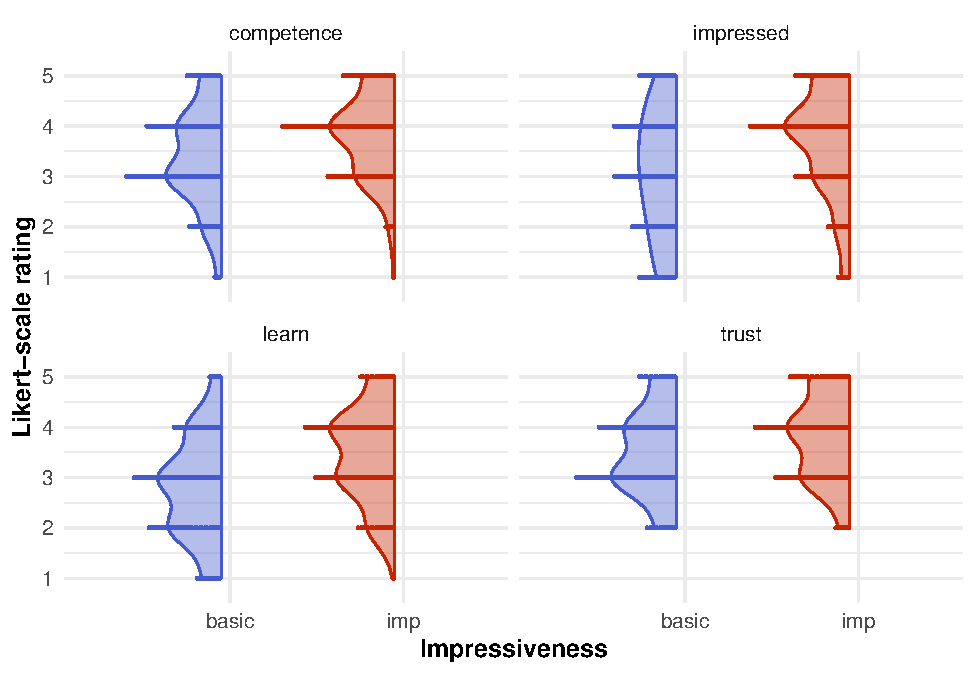
\includegraphics{output/figures/exp1-plot.pdf}
\caption{\label{fig:exp1-plot}Overview of treatment effect on various outcomes}
\end{figure}

\newpage

\hypertarget{experiment-2}{%
\section{Experiment 2}\label{experiment-2}}

Experiment 2 is essentially intended to be a slightly improved replication of experiment 1.

Although we confirmed all our hypotheses, there were a couple of issues with experiment 1 that make us feel that a replication is warranted (see Procedure and materials)

\hypertarget{methods-1}{%
\subsection{Methods}\label{methods-1}}

\hypertarget{participants-1}{%
\subsubsection{Participants}\label{participants-1}}

We recruited 100 participants via Prolific. One participant failed our attention check and one had NA scores for all outcomes, so we decided to remove them, resulting in a final sample of 99 participants (49 female, 50 male; \(age_\text{mean}\): 42.07, \(age_\text{sd}\): 12.86, \(age_\text{median}\): 40).

\hypertarget{procedure-and-materials}{%
\subsubsection{Procedure and materials}\label{procedure-and-materials}}

The design of study 2 will be identical to the design of study 1 but we corrected a couple of issues :

\begin{itemize}
\item
  We made a technical mistake : For both the impressive and basic entomology stimuli, our manipulation check question read: ``How impressive do you think the findings of the archeologists described in the text are?'', whereas it should have read ``\ldots{} the findings of entomologists\ldots{}''. Two participants brought this issue to our attention. While it should not have affected Hypotheses 1a and 2a, it might have distorted results on Hypotheses 1b and 2b which rely on the faulty question item. We will correct this mistake for study 2.
\item
  One participant remarked that we should have spelled ``archaeology'' instead of ``archeology''. To avoid potential confusion, we will change the spelling accordingly for study 2.
\item
  Regarding our archeology vignettes--contrary to the findings in our pilot study--participants did not rate the impressive version more impressive than the basic version. We will therefore use slightly modified vignettes for archeology for study 2, hoping to make the two conditions more distinguishable. We also shortened the text in both conditions to be more similar in length to (i) each other and (ii) to the entomology vignettes. In Appendix \ref{exp1}, Table \ref{tab:stimuli} show the old version from study 1 and the new version for study 2.
\end{itemize}

We will also run the study on UK participants, using the opportunity of replicating the main results on a different population sample.

\hypertarget{results-1}{%
\subsection{Results}\label{results-1}}

Results are similar to experiment 1 which confirm our studies.

For a manipulation check, we find that--in line with pilot studies--participants indeed perceive the impressive text as more impressive (mean = 4.01, sd = 0.87; \(\hat{b}\) = 0.81 {[}0.569, 1.048{]}, p \textless{} .001) than the basic text (mean = 3.20, sd = 1.13).

We find that participants perceive scientists as more competent after having read an impressive text (mean = 3.76, sd = 0.90; \(\hat{b}_{\text{Competence}}\) = 0.50 {[}0.314, 0.676{]}, p \textless{} .001) than after having read a basic one (mean = 3.26, sd = 0.80). Pooled across all conditions, participants impressiveness ratings are positively associated with competence (\(\hat{b}\) = 0.41 {[}0.312, 0.502{]}, p \textless{} .001).

Similar to competence, we find that participants trust a discipline more after having read an impressive text (mean = 3.68, sd = 0.87; \(\hat{b}_{\text{trust}}\) = 0.32 {[}0.17, 0.476{]}, p \textless{} .001) than after having read a basic one. Participants impressiveness ratings are positively associated with trust when pooling across all conditions (\(\hat{b}\) = 0.30 {[}0.206, 0.385{]}, p \textless{} .001).

For RQ1, we find that participants had the impression of having learned after having read the impressive text (mean = 3.66, sd = 0.93; \(\hat{b}\) = 0.89 {[}0.67, 1.108{]}, p \textless{} .001), than after having read the basic one ((mean = 2.77, sd = 0.96).

Regarding RQ2, we do not find evidence that consensus modulates the effect of impressiveness hypothesized in H1a and H2a.

Fig. \ref{fig:exp2-plot} summarizes descriptive results. In Appendix \ref{exp2}, we provide regression tables and additional analyses.



\begin{figure}
\centering
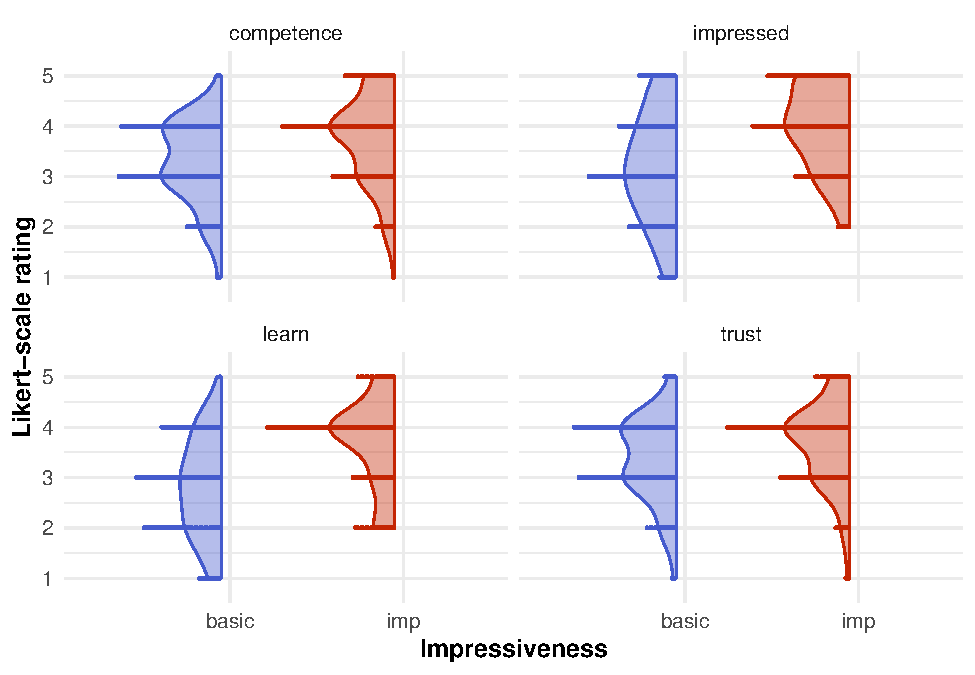
\includegraphics{output/figures/exp2-plot.pdf}
\caption{\label{fig:exp2-plot}Overview of treatment effect on various outcomes}
\end{figure}

\FloatBarrier

\hypertarget{references}{%
\section{References}\label{references}}

\hypertarget{refs}{}
\begin{CSLReferences}{1}{0}
\leavevmode\vadjust pre{\hypertarget{ref-colognaTrustClimateScience2023}{}}%
Cologna, V., Kotcher, J., Mede, N. G., Besley, J., Maibach, E., \& Oreskes, N. (n.d.). \emph{Trust in climate science and climate scientists: A qualitative review}. \url{https://doi.org/10.31234/osf.io/hj2xk}

\end{CSLReferences}

\newpage

\hypertarget{appendix-appendix}{%
\appendix}


\hypertarget{exp1}{%
\section{Experiment 1}\label{exp1}}

\hypertarget{materials-1}{%
\subsection{Materials}\label{materials-1}}

\FloatBarrier

\hypertarget{descriptives}{%
\subsection{Descriptives}\label{descriptives}}

\begin{table}
\centering\centering
\caption{\label{tab:exp1-descriptives}Descriptives}
\centering
\resizebox{\ifdim\width>\linewidth\linewidth\else\width\fi}{!}{
\begin{tabular}[t]{llrrrrr}
\toprule
discipline & impressiveness & impressed\_mean & learn\_mean & competence\_mean & trust\_mean & consensus\_mean\\
\midrule
archeo & basic & 3.71 & 3.10 & 3.45 & 3.61 & 4.08\\
archeo & imp & 3.67 & 3.18 & 3.63 & 3.61 & 3.88\\
entom & basic & 2.43 & 2.49 & 3.35 & 3.39 & 3.98\\
entom & imp & 3.65 & 3.78 & 4.02 & 4.02 & 3.78\\
\bottomrule
\end{tabular}}
\end{table}

\hypertarget{regression-tables}{%
\subsection{Regression tables}\label{regression-tables}}

The results of the models from the hypotheses can be found in table \ref{tab:exp1-hypotheses-table}.

\begin{table}
\centering\centering
\resizebox{\ifdim\width>\linewidth\linewidth\else\width\fi}{!}{
\begin{tabular}[t]{lcccc}
\toprule
  & H1a (Competence) & H1b (Competence pooled) & H2a (Trust) & H2b (Trust pooled)\\
\midrule
(Intercept) & 3.263*** & 2.043*** & 3.354*** & 2.449***\\
 & (0.086) & (0.185) & (0.086) & (0.177)\\
impressivenessimp & 0.495*** &  & 0.323*** & \\
 & (0.091) &  & (0.077) & \\
impressed &  & 0.407*** &  & 0.296***\\
 &  & (0.048) &  & (0.045)\\
SD (Intercept id) & 0.565 & 0.409 & 0.657 & 0.551\\
SD (Observations) & 0.642 & 0.640 & 0.542 & 0.547\\
\midrule
Num.Obs. & 198 & 198 & 198 & 198\\
R2 Marg. & 0.078 & 0.254 & 0.035 & 0.147\\
R2 Cond. & 0.480 & 0.471 & 0.609 & 0.577\\
AIC & 491.4 & 458.1 & 467.9 & 446.7\\
BIC & 504.5 & 471.3 & 481.0 & 459.9\\
ICC & 0.4 & 0.3 & 0.6 & 0.5\\
RMSE & 0.53 & 0.56 & 0.43 & 0.44\\
\bottomrule
\multicolumn{5}{l}{\rule{0pt}{1em}+ p $<$ 0.1, * p $<$ 0.05, ** p $<$ 0.01, *** p $<$ 0.001}\\
\end{tabular}}
\end{table}

The results of the model from RQ1 and of the models from RQ2 (interaction between impressiveness and consensus on competence/trust) can be found in table \ref{tab:exp1-consensus-table}.

\begin{table}
\centering\centering
\resizebox{\ifdim\width>\linewidth\linewidth\else\width\fi}{!}{
\begin{tabular}[t]{lccccc}
\toprule
  & RQ 1 & H1a x Consensus & H1b x Consensus & H2a x Consensus & H2b x Consensus\\
\midrule
(Intercept) & 2.768*** & 2.904*** & 1.899** & 3.287*** & 2.965***\\
 & (0.095) & (0.346) & (0.647) & (0.375) & (0.681)\\
impressivenessimp & 0.889*** & 0.132 &  & -0.371 & \\
 & (0.110) & (0.398) &  & (0.456) & \\
consensus &  & 0.117 & 0.153 & -0.006 & -0.250\\
 &  & (0.087) & (0.168) & (0.095) & (0.179)\\
impressivenessimp × consensus &  & 0.054 &  & 0.230+ & \\
 &  & (0.103) &  & (0.118) & \\
impressed &  &  & 0.391* &  & 0.129\\
 &  &  & (0.187) &  & (0.194)\\
impressed × consensus &  &  & -0.027 &  & 0.074\\
 &  &  & (0.048) &  & (0.050)\\
SD (Intercept id) & 0.535 & 0.634 & 0.552 & 0.547 & 0.390\\
SD (Observations) & 0.775 & 0.548 & 0.548 & 0.641 & 0.648\\
\midrule
Num.Obs. & 198 & 198 & 198 & 198 & 198\\
R2 Marg. & 0.183 & 0.056 & 0.155 & 0.101 & 0.262\\
R2 Cond. & 0.447 & 0.596 & 0.581 & 0.480 & 0.458\\
AIC & 539.3 & 473.5 & 457.3 & 495.0 & 467.7\\
BIC & 552.4 & 493.2 & 477.0 & 514.7 & 487.4\\
ICC & 0.3 & 0.6 & 0.5 & 0.4 & 0.3\\
RMSE & 0.67 & 0.43 & 0.44 & 0.53 & 0.57\\
\bottomrule
\multicolumn{6}{l}{\rule{0pt}{1em}+ p $<$ 0.1, * p $<$ 0.05, ** p $<$ 0.01, *** p $<$ 0.001}\\
\end{tabular}}
\end{table}

\newpage

\hypertarget{exp2}{%
\section{Experiment 2}\label{exp2}}

\hypertarget{materials-2}{%
\subsection{Materials}\label{materials-2}}

\FloatBarrier

\hypertarget{descriptives-1}{%
\subsection{Descriptives}\label{descriptives-1}}

\begin{table}
\centering\centering
\caption{\label{tab:exp2-descriptives}Descriptives}
\centering
\resizebox{\ifdim\width>\linewidth\linewidth\else\width\fi}{!}{
\begin{tabular}[t]{llrrrrr}
\toprule
discipline & impressiveness & impressed\_mean & learn\_mean & competence\_mean & trust\_mean & consensus\_mean\\
\midrule
archeo & basic & 3.31 & 2.78 & 3.31 & 3.35 & 3.90\\
archeo & imp & 3.98 & 3.48 & 3.70 & 3.60 & 3.92\\
entom & basic & 3.10 & 2.76 & 3.22 & 3.36 & 3.78\\
entom & imp & 4.04 & 3.84 & 3.82 & 3.76 & 3.59\\
\bottomrule
\end{tabular}}
\end{table}

\hypertarget{regression-tables-1}{%
\subsection{Regression tables}\label{regression-tables-1}}

The results of the models from the hypotheses can be found in table \ref{tab:exp2-hypotheses-table}.

\begin{table}
\centering\centering
\resizebox{\ifdim\width>\linewidth\linewidth\else\width\fi}{!}{
\begin{tabular}[t]{lcccc}
\toprule
  & H1a (Competence) & H1b (Competence pooled) & H2a (Trust) & H2b (Trust pooled)\\
\midrule
(Intercept) & 3.263*** & 2.043*** & 3.354*** & 2.449***\\
 & (0.086) & (0.185) & (0.086) & (0.177)\\
impressivenessimp & 0.495*** &  & 0.323*** & \\
 & (0.091) &  & (0.077) & \\
impressed &  & 0.407*** &  & 0.296***\\
 &  & (0.048) &  & (0.045)\\
SD (Intercept id) & 0.565 & 0.409 & 0.657 & 0.551\\
SD (Observations) & 0.642 & 0.640 & 0.542 & 0.547\\
\midrule
Num.Obs. & 198 & 198 & 198 & 198\\
R2 Marg. & 0.078 & 0.254 & 0.035 & 0.147\\
R2 Cond. & 0.480 & 0.471 & 0.609 & 0.577\\
AIC & 491.4 & 458.1 & 467.9 & 446.7\\
BIC & 504.5 & 471.3 & 481.0 & 459.9\\
ICC & 0.4 & 0.3 & 0.6 & 0.5\\
RMSE & 0.53 & 0.56 & 0.43 & 0.44\\
\bottomrule
\multicolumn{5}{l}{\rule{0pt}{1em}+ p $<$ 0.1, * p $<$ 0.05, ** p $<$ 0.01, *** p $<$ 0.001}\\
\end{tabular}}
\end{table}

The results of the model from RQ1 and of the models from RQ2 (interaction between impressiveness and consensus on competence/trust) can be found in table \ref{tab:exp2-consensus-table}.

\begin{table}
\centering\centering
\resizebox{\ifdim\width>\linewidth\linewidth\else\width\fi}{!}{
\begin{tabular}[t]{lccccc}
\toprule
  & RQ 1 & H1a x Consensus & H1b x Consensus & H2a x Consensus & H2b x Consensus\\
\midrule
(Intercept) & 2.768*** & 2.904*** & 1.899** & 3.287*** & 2.965***\\
 & (0.095) & (0.346) & (0.647) & (0.375) & (0.681)\\
impressivenessimp & 0.889*** & 0.132 &  & -0.371 & \\
 & (0.110) & (0.398) &  & (0.456) & \\
consensus &  & 0.117 & 0.153 & -0.006 & -0.250\\
 &  & (0.087) & (0.168) & (0.095) & (0.179)\\
impressivenessimp × consensus &  & 0.054 &  & 0.230+ & \\
 &  & (0.103) &  & (0.118) & \\
impressed &  &  & 0.391* &  & 0.129\\
 &  &  & (0.187) &  & (0.194)\\
impressed × consensus &  &  & -0.027 &  & 0.074\\
 &  &  & (0.048) &  & (0.050)\\
SD (Intercept id) & 0.535 & 0.634 & 0.552 & 0.547 & 0.390\\
SD (Observations) & 0.775 & 0.548 & 0.548 & 0.641 & 0.648\\
\midrule
Num.Obs. & 198 & 198 & 198 & 198 & 198\\
R2 Marg. & 0.183 & 0.056 & 0.155 & 0.101 & 0.262\\
R2 Cond. & 0.447 & 0.596 & 0.581 & 0.480 & 0.458\\
AIC & 539.3 & 473.5 & 457.3 & 495.0 & 467.7\\
BIC & 552.4 & 493.2 & 477.0 & 514.7 & 487.4\\
ICC & 0.3 & 0.6 & 0.5 & 0.4 & 0.3\\
RMSE & 0.67 & 0.43 & 0.44 & 0.53 & 0.57\\
\bottomrule
\multicolumn{6}{l}{\rule{0pt}{1em}+ p $<$ 0.1, * p $<$ 0.05, ** p $<$ 0.01, *** p $<$ 0.001}\\
\end{tabular}}
\end{table}

\hypertarget{stimuli}{%
\subsection{Stimuli}\label{stimuli}}

\begin{longtable}[t]{>{\raggedright\arraybackslash}p{5em}>{\raggedright\arraybackslash}p{20em}>{\raggedright\arraybackslash}p{20em}}
\caption{\label{tab:stimuli}Stimuli}\\
\toprule
 & Experiment 1 (old) & Experiment 2 (new)\\
\midrule
basic & Archaeology is the science that studies human history and prehistory based on the analysis of objects from the past such as human bones, engravings, constructions, and various objects, from nails to bits of pots. This task requires a great deal of carefulness, because objects from the past need to often be dug out from the ground and cleaned, without destroying them in the process. 

Archeologists have been able to shed light on human history in all continents, from ancient Egypt to the Incas in Peru or the Khmers in Cambodia. 

Archaeologists have made some startling discoveries, such as the amazing animal paintings in the Lascaux caves, which have been shown to be at least 30000 years old. On that basis, archeologists speculate on the artistic and religious lives of our ancestors. 

Archeologists have also been able to find remains of our more distant ancestors, showing that our species is just one among several that appeared and then went extinct, such as Neanderthals, Homo erectus, or Homo habilis. 

Archaeology relies on scientific methods of analysis such as carbon dating, which enables us to date objects, based on the type of carbon atoms they contain. & Archaeology is the science that studies human history and prehistory based on the analysis of objects from the past such as human bones, engravings, constructions, and various objects, from nails to bits of pots. This task requires a great deal of carefulness, because objects from the past need to often be dug out from the ground and patiently cleaned, without destroying them in the process.

Archaeologists have been able to shed light on human history in all continents, from ancient Egypt to the Incas in Peru or the Khmers in Cambodia.

Archaeologists study the paintings made by our ancestors, such as those that can be found in Lascaux, a set of caves found in the south of France that have been decorated by people at least 30000 years ago.

Archaeologists have also found remains of our more distant ancestors, showing that our species is just one among several that appeared, and then either changed or went extinct, such as Neanderthals, Homo erectus, or Homo habilis.\\
impressive & Archeologists, scientists who study human history and prehistory, are able to tell, from their bones, whether someone was male or female, how old they were, and whether they suffered from a wide range of diseases. Archeologists can now even tell at what age someone, dead for tens of thousands of years, stopped drinking their mother’s milk, from the composition of their teeth. 

Looking for patterns, archeologists can also understand how far our ancestors traveled, or how often they fought each other.

Archeologists can learn about the language that our ancestors or cousins might have had. For instance, the nerve that is used to control breathing is larger in humans than in apes, plausibly because we need more fine-grained control of our breathing in order to speak. As a result, the canal containing that nerve is larger in humans than in apes – and it is also enlarged in Neanderthals. 

We can also tell, from an analysis of the tools they made, that, like modern humans, most Neanderthals were right-handed. It’s thought that handedness is related to the evolution of language, another piece of evidence suggesting that Neanderthals likely possessed a form of language. & Archaeologists, scientists who study human history and prehistory, are able to tell, from their bones, whether someone was male or female, how old they were, and whether they suffered from a range of diseases. Archaeologists can now tell at what age someone, dead for tens of thousands of years, stopped drinking their mother’s milk, from the composition of their teeth.
Archaeologists learn about the language that our ancestors or cousins might have had. For instance, the nerve that is used to control breathing is larger in humans than in apes, plausibly because we need more fine-grained control of our breathing in order to speak. As a result, the canal containing that nerve is larger in humans than in apes – and it is also enlarged in Neanderthals.
Archaeologists can also tell, from an analysis of the tools they made, that most Neanderthals were right-handed. It’s thought that handedness is related to the evolution of language, another piece of evidence suggesting that Neanderthals likely possessed a form of language.\\
\bottomrule
\end{longtable}

\newpage

\hypertarget{pilot}{%
\section{Preceding pilot}\label{pilot}}

Avant chacune de nos expérimentations, nous avons effectué des ``pilots'' pour tester


\end{document}
